%Mall skapad av Andréas Sundström, Göteborg, 2015-02-28.
%Neders i filen finns lite påminnelser om hur man använder vissa
%kommandon. 

%Grunden är baserad på Christian von Schults mall.
\documentclass[12pt,a4paper]{article}
\pdfoutput=1
%%%%%%%%%%%%%%%%%%%%%%%vons grund%%%%%%%%%%%%%%%%%%%%%%%
\usepackage[utf8]{inputenc}
\usepackage[T1]{fontenc}
\usepackage[swedish]{babel} %OBS! Se till att vi får rätt språk.
\usepackage{amsmath}
\usepackage{lmodern}
\usepackage{units}
\usepackage{icomma}
\usepackage{color}
\usepackage{graphicx}
\usepackage{bbm}
\newcommand{\N}{\ensuremath{\mathbbm{N}}}
\newcommand{\Z}{\ensuremath{\mathbbm{Z}}}
\newcommand{\Q}{\ensuremath{\mathbbm{Q}}}
\newcommand{\R}{\ensuremath{\mathbbm{R}}}
\newcommand{\C}{\ensuremath{\mathbbm{C}}}
\newcommand{\rd}{\ensuremath{\mathrm{d}}}
\newcommand{\id}{\ensuremath{\,\rd}}
\usepackage{hyperref}

%%%%%%%%%%%%%%%%%%%%%%%Egna tillägg%%%%%%%%%%%%%%%%%%%%%%%

%%Partiell derivata
\newcommand{\pd}{\ensuremath{\partial}}
%%Följer ISO-8601 oberoende av språk.
\usepackage{datetime} 
\newdateformat{specialdate}{\THEYEAR-\twodigit{\THEMONTH}-\twodigit{\THEDAY}}
%%Göra grader Celcius
\newcommand{\degC}{\ensuremath{\,^\circ\mathrm{C}}}
%%Figurreferenser
\newcommand{\Figref}{\figurename~\ref} %Stor bokstav i början
\newcommand{\figref}{\MakeLowercase{\figurename}~\ref} 
%%Tabellreferenser
\newcommand{\Tabref}{\tablename~\ref} %Stor bokstav i början
\newcommand{\tabref}{\MakeLowercase{\tablename}~\ref}
%%Ohm enhetskommando
\newcommand{\ohm}{\ifmmode \Omega \else $\Omega$ \fi}
%%Varepsilon är det enda rätta epsilon
\renewcommand{\epsilon}{\varepsilon}


%%%%%%%%%%%%%%%%%%Övriga matnyttiga paket%%%%%%%%%%%%%%%%%

%%För att kunna inkludera andra PDF-dokument
\usepackage{pdfpages}
%%För att kunna ha roterade bilder
\usepackage{rotating}
%%För att inkludera MATLABkod. 
%\usepackage[framed,numbered,autolinebreaks,useliterate]{mcode}
%\usepackage{listings} 
%\lstloadlanguages{matlab} 
%\lstset{language=matlab} 
%\lstset{literate= {å}{{\r{a}}}1 {ä}{{\"a}}1 {ö}{{\"o}}1 {Å}{{\r{A}}}1
%  {Ä}{{\"A}}1 {Ö}{{\"O}}1}%För att få svenska bokstäver från MATLAB.


%%För att själv bestämma marginalerna. 
%\usepackage[
%            top    = 3cm,
%            bottom = 3cm,
%            left   = 3cm, right  = 3cm
%]{geometry}




%Fixar typstorleken i \section så att den inte blir för stor
\usepackage{sectsty}
\sectionfont{\fontsize{13}{0}\selectfont}

\begin{document}
\title{Resistanstråd}
\author{}
\date{}%Datum för experimentfinal 2015
\maketitle

% %Jag tänker mig att numrering är onödig
% \section*{Bakgrund} 
% %Det kan vara bra med en kort bakrund (typ 50-75 ord).
% %Ska det vara några bilder här? Det känns mest störiga.
% Alla material uppvisar längdutvidgning, och i begränsade
% temperaturintervall kan längdutvidgningen antas vara linjär:
% \[l=l_0(1+\alpha\Delta T), \]
% där $\Delta T = T-T_0$ är temperaturskillnaden, $l$ är den aktuella
% längden, $l_0$ är längden vid temperaturen $T=T_0$, och $\alpha$ är
% materialets längdutvidgningskoefficient. Det är dock svårt att
% observera längdutvidgning i vardagen då den är så liten, men några
% exempel är sprittermometrar, järnvägsräls och broar.

% \section*{Uppgift}
%Ha med relevanta bilder
%Tilltal i singular: ''Din uppgift är att ...''
Alla material uppvisar längdutvidgning, och i begränsade
temperaturintervall kan längdutvidgningen antas vara linjär:
\[l=l_0(1+\alpha\Delta T), \]
där $\Delta T = T-T_0$ är temperaturskillnaden, $l$ är den aktuella
längden, $l_0$ är längden vid temperaturen $T=T_0$, och $\alpha$ är
materialets längdutvidgningskoefficient.

Värmeöverföring genom en yta lyder följande samband:
\[ P = k \Delta T, \]
där $P$ är bortledd värmeeffekt,
$\Delta T$ är temperaturskillnaden i ytan och $k$ är en konstant.

Du har fått en resistanstråd. Din uppgift är nu att:
\begin{enumerate}
\item använd värmeöverföringsekvationen för att avgöra vilken typ av
  samband som borde gälla mellan trådtemperaturen, $T$, och strömmen, $i$, genom
  tråden. (Alltså på vilket sätt som $T$ teoretiskt beror av $i$ givet
  vissa konstanter.)
\item bestämma trådtemperaturen som funktion av strömmen genom
  tråden, svara med en graf. \\ 
\large
OBS: Ta \textbf{INTE} i tråden när det går ström genom den! Den är 
varm!
\normalsize 
\item förklara varför/varför inte något fattas det i det samband som
  du tog fran i 1? (Du behöver inte ta fram något nytt samband, bara
  förklara och motivera om det är något mer som borde tas med i
  beräkningen.) 
% \item förklara, med data från dina mätningar, vad som fattas när du
%   tog fram sambandet i uppgift 1.

% \item beräkna konstanten, $k$, i värmeöverföringsekvationen ovan för
%   en 1~m lång trådbit ($k$ beror linjärt med längden, $L$, av tråden:
%   $k=\text{konst.}\times L$).
\end{enumerate}



%\emph{Fysiktips 2}: Vad är den tillförda effekten till tråden?

\emph{Mattetips}: För $h\ll d$ ($h$ mycket\footnotemark mindre än $d$)
kan man göra följande  approximation:
\[ \sqrt{d^2+h^2} = d\sqrt{1+\frac{h^2}{d^2}} 
\approx d\left( 1+\frac{h^2}{2d^2}\right). \]
\footnotetext{Det brukar räcka med $h \le d/10$ för att få en mycket
  god approximation.}

\section*{Materiel}
%Lista all utrustning. Vid behöv förklara den.
%Här måste vi ha med bilder på all utrustning!

%En punktlista med all materiel.
%Listan bör innehålla: <antal>, <sak>, <ev. förklaring hur den
%används>

\begin{itemize}
\item 1,5~m resistanstråd\\% av typ RD 100/0,2. 
  Nedan följer lite fakta om tråden.
\begin{itemize}
\item Den har en längdutvidgningskoefficient på
  $\alpha=\unit[13,5\times 10^{-6}]{K^{-1}}$.
\item Den har försumbar resistansförändring i det temperaturintervall
  som vi jobbar i.
\item Tråddiametern är 0,2~mm.
\end{itemize}
\item 5~cm ståltråd
\item 2 st. skruvtvingar
\item Spänningsaggregat
\item Multimeter
\item Labbsladdar med krokodilklämmor\footnotemark
\item Termometer
\item Tumstock och linjal
\item En linjal med ståltrådskrok
\end{itemize}
\footnotetext{Obs: det kan vara svårt att få kontakt mellan tråden och
  krokodilklämmorna p.g.a. ett tunnt oxidskikt. Vicka lite på klämmorna
  när de sitter på tråden eller skrapa lite lätt på tråden om du
  upplever att det inte blir ordentlig kontakt.}
Några saker att tänka på med tråden:\\
Kör inte mer än 2~A genom tråden, den blir då för varm och börjar
oxidera. \\
Dra inte för hårt i tråden; den kommer att töjas ut. 

Om du råkar göra något av det ovanstående bör du be handledaren om en
ny tråd. Detta kommer att noteras, och kan påverka din poäng.

\begin{figure}\centering
\centerline{ %centrerar även större bilder
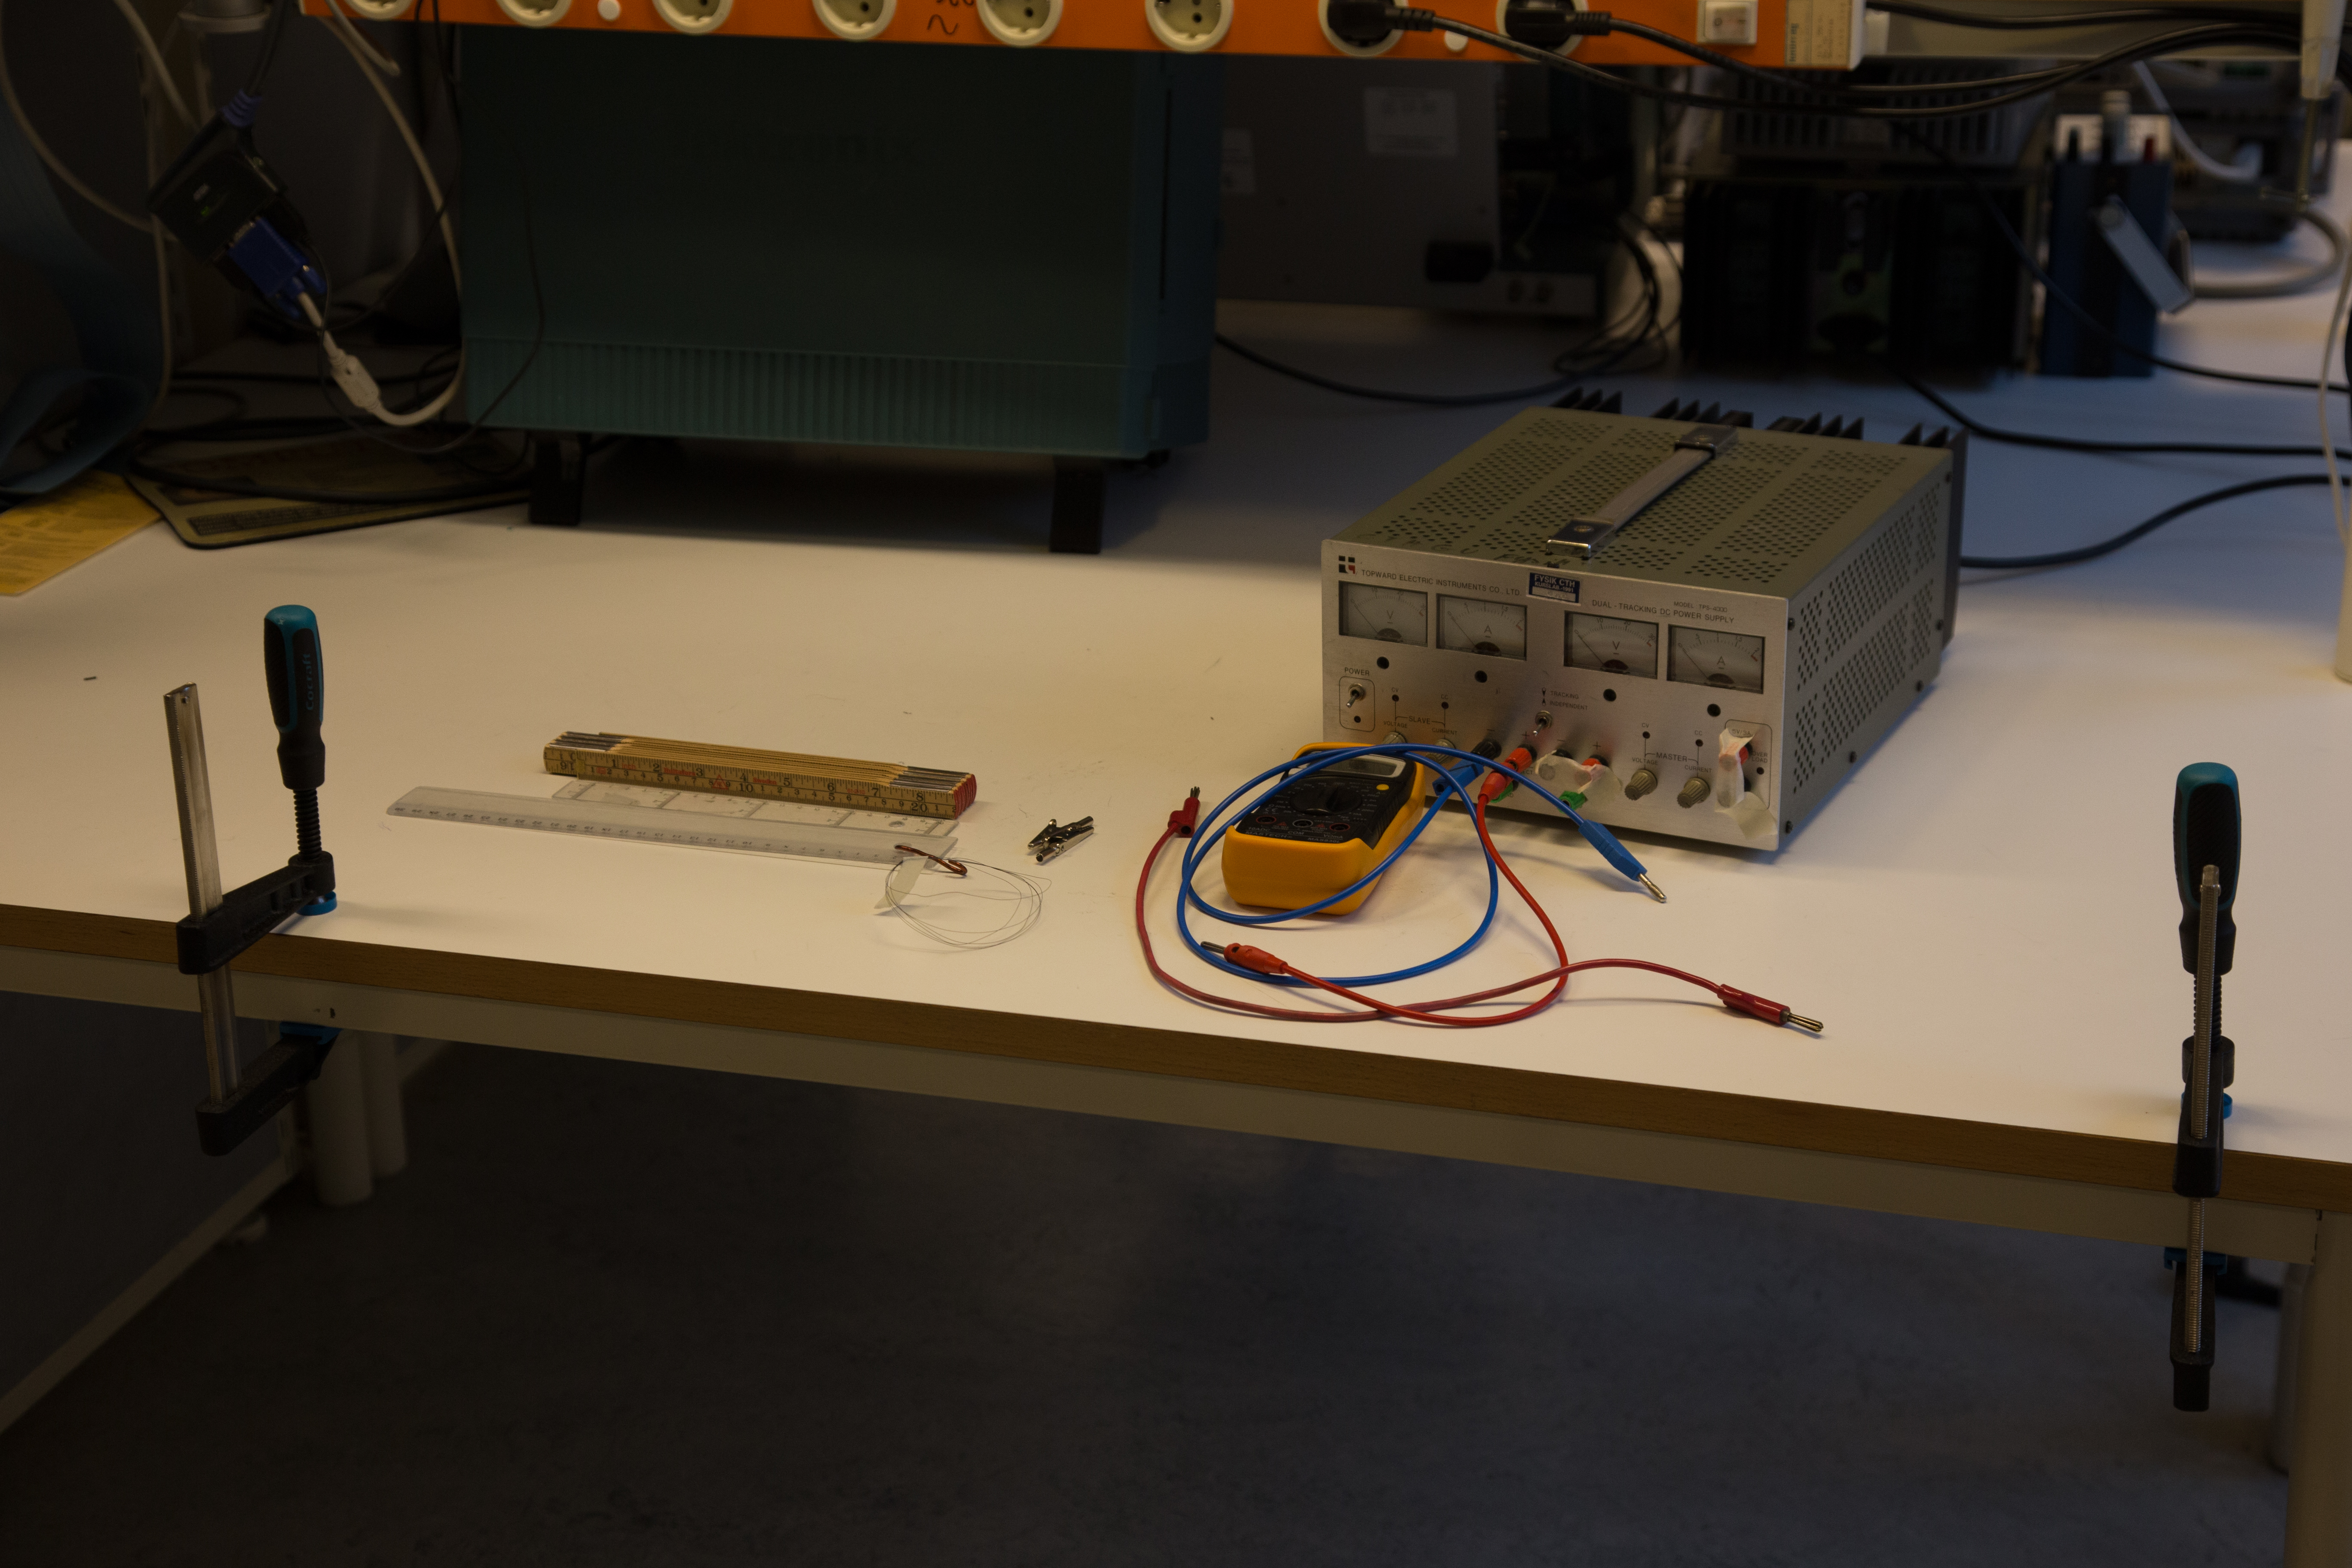
\includegraphics[width=1\textwidth]{IMG_3588.jpg}
}
%\caption{\label{figuren} Perioden $T$ som funktion av pendellängden.}
\end{figure}

\end{document}
%%%%%%%%Påminnelser om hur man använder vissa kommandon%%%%%%%%%%

%% På svenska ska citattecknet vara samma i både början och slut.
%% Använd två apostrofer (två enkelfjongar): ''.

%%För att referera till till tidigare fotnot:
%\footnotemark[\value{footnote}]

%% Inkludera PDF-dokument
%\includepdf[pages={1-}]{filnamn.pdf} %Filnamnet får INTE innehålla 'mellanslag'!

%% Figurer inkluderade som pdf-filer
%\begin{figure}\centering
%\centerline{ %centrerar även större bilder
%\includegraphics[width=1\textwidth]{filnamn.pdf}
%}
%\caption{\label{figuren} Perioden $T$ som funktion av pendellängden.}
%\end{figure}

%% Figurer inkluderade med xfigs "Combined PDF/LaTeX"
%\begin{figure}\centering
%\input{filnamn.pdf_t}
%\caption{\label{finafiguren} Perioden $T$ som funktion av
%  pendellängden.}
%\end{figure}


%% Figurer roterade 90 grader
%\begin{sidewaysfigure}\centering
%\centerline{ %centrerar även större bilder
%\includegraphics[width=1\textwidth]{filnamn.pdf}
%}
%\caption{\label{figuren} Perioden $T$ som funktion av pendellängden.}
%\end{sidewaysfigure}
